\section{How Ethical Issues are Addressed}

There are no ethical issues involved with this project, as no personal data is being used in either the design, implementation or evaluation of the solution. All data used for evaluation is either synthetic data generated specifically for this project or publicly available datasets.

\section{Supplementary Material}

\begin{figure}[H]
	\centering
	\includegraphics[scale=0.6]{figures/full-project-process.pdf}
	\caption{Flow Chart of Full Project Schedule}
	\label{fig:full-project-process}
\end{figure}

\newpage

\null  % Empty line
\nointerlineskip  % No skip for prev line
\vfill
\let\snewpage \newpage
\let\newpage \relax

\begin{figure}[H]
	\centering
	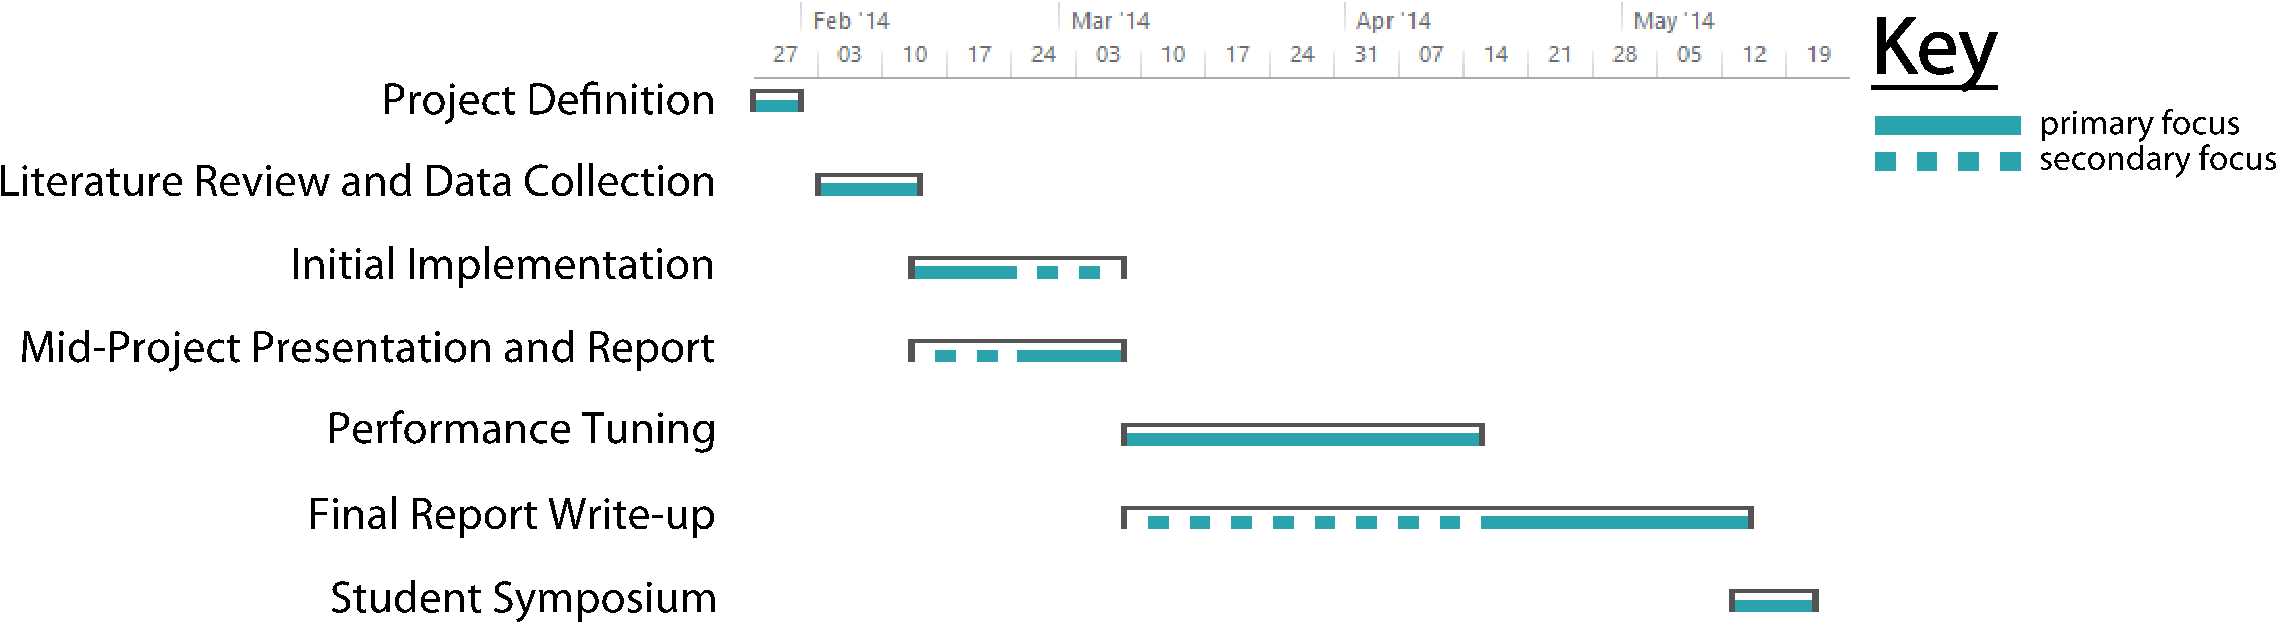
\includegraphics[scale=0.475]{figures/initial_project_schedule.pdf}
	\caption{Initial Project Schedule Created on 31/01/14. The time this report was submitted is marked on the chart to illustrate the project's current progress.}
	\label{fig:initial-schedule}
\end{figure}

\begin{figure}[H]
	\centering
	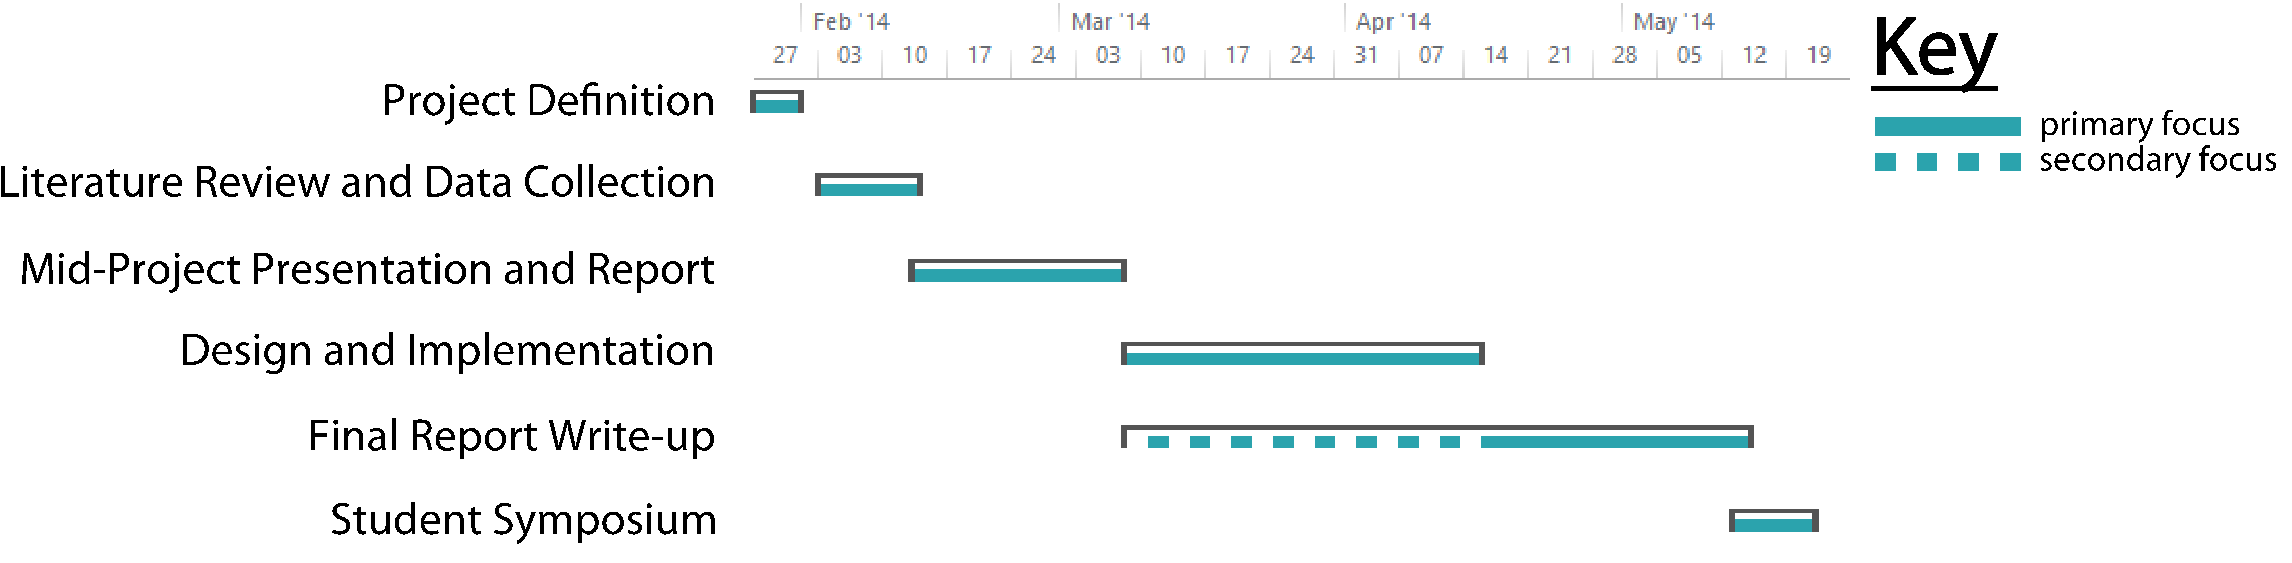
\includegraphics[scale=0.475]{figures/revised_project_schedule.pdf}
	\caption{Revised Project Schedule Created on 20/02/14. The time this report was submitted is marked on the chart to illustrate the project's current progress.}
	\label{fig:revised-schedule}
\end{figure}

\let \newpage \snewpage
\vfill 
\break % page break

\begin{landscape}	

\null  % Empty line
\nointerlineskip  % No skip for prev line
\vfill
\let\snewpage \newpage
\let\newpage \relax
	\begin{figure}[H]
		\centering
		\includegraphics[scale=0.35]{figures/md_structure_taxonomy.png}
		\caption{Multi-dimensional Search Structure Taxonomy}
		\label{fig:structure-taxonomy}
	\end{figure}
\let \newpage \snewpage
\vfill 
\break % page break

	\newpage

\null  % Empty line
\nointerlineskip  % No skip for prev line
\vfill
\let\snewpage \newpage
\let\newpage \relax
	\begin{figure}[H]
		\centering
		\centerline{ 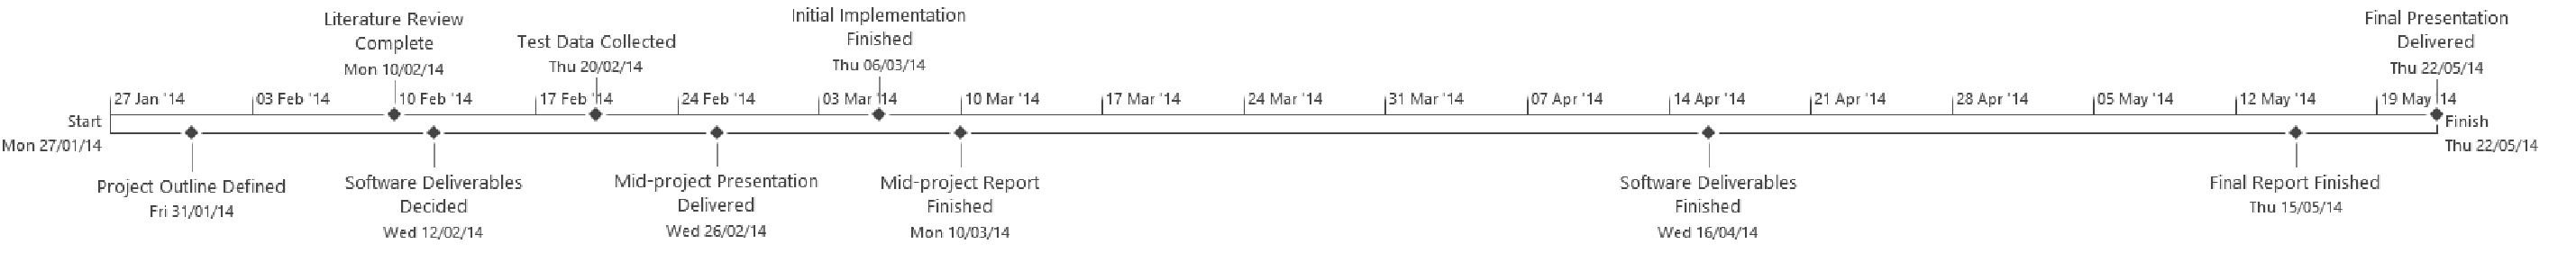
\includegraphics[scale=0.5]{figures/initial_schedule_timeline.pdf} }
		\caption{Initial Milestone Timeline Created on 20/02/14}
		\label{fig:initial-milestone-timeline}
	\end{figure}

	\begin{figure}[H]
		\centering
		\centerline{ 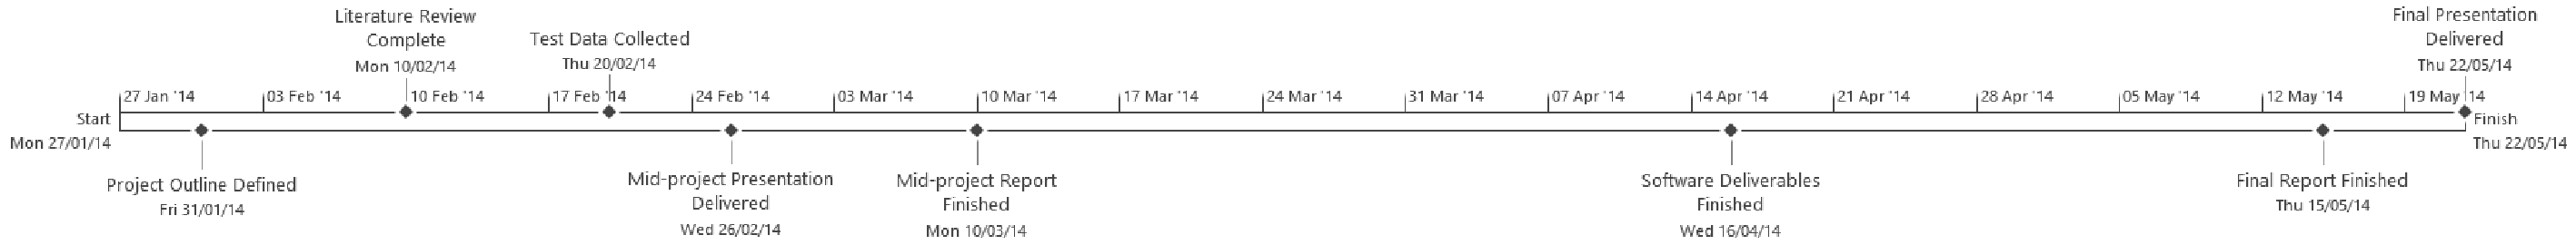
\includegraphics[scale=0.37]{figures/revised_schedule_timeline.pdf} }
		\caption{Revised Milestone Timeline Created on 20/02/14}
		\label{fig:revised-milestone-timeline}
	\end{figure}	
\let \newpage \snewpage
\vfill 
\break % page break

\end{landscape}

\begin{table}
	\centering
	\begin{tabular}{|p{2.8cm}|p{2.3cm}|p{3cm}|p{3cm}|p{3.5cm}|p{2cm}|}
		\hline
		\textbf{Index Structure} &
		\textbf{Memory Overhead} &
		\textbf{Bucket Method?} &
		\textbf{High-Dimensional Data} &
		\textbf{Complexity} \\
		\hline
		Sequential Scan & Low & No (but since data is stored contiguously, there are minimal I/O operations due to sequential access) & Often better than other structures with high $d$ (but significantly poorer performance with low $d$) & Low \\		
		B${}^{+}$-Tree & Low & Yes & One-dimensional & Low \\
		R-Tree & Moderate & Yes & Poor for $d > 10$ \cite{pyramid-tree} & Moderate \\
		Quadtree & Low with uniformly distributed data, high for skewed data due to unnecessary nodes caused by splitting sparse regions of data space & No & Poor because it tries to use balanced splits \cite{pyramid-tree} & Low \\
		Pyramid Tree & Low & Yes (based on B${}^{+}$-tree) & Good & High \\
		PK-Tree & Moderate & No (but uses similar method to reduce I/O operations) & Good & High \\
		Skip Quadtree & Moderate & No & Untested & Moderate \\
		Quadtreap & Low & No & Untested & Moderate \\
		Splay Quadtree & Moderate & No & Untested & Moderate \\
		\hline
	\end{tabular}
	\caption{Comparison of Dynamic Multi-Dimensional Structures}
	\label{tab:comparison}
\end{table}

